\documentclass[a4paper,journal]{IEEEtran}
\usepackage[utf8]{inputenc}
\usepackage[brazil]{babel}
\usepackage{amssymb}

\newcommand{\specialcell}[2][c]{%
  \begin{tabular}[#1]{@{}c@{}}#2\end{tabular}}

\usepackage{graphics}

% Some very useful LaTeX packages include:
% (uncomment the ones you want to load)


% *** MISC UTILITY PACKAGES ***
%
%\usepackage{ifpdf}
% Heiko Oberdiek's ifpdf.sty is very useful if you need conditional
% compilation based on whether the output is pdf or dvi.
% usage:
% \ifpdf
%   % pdf code
% \else
%   % dvi code
% \fi
% The latest version of ifpdf.sty can be obtained from:
% http://www.ctan.org/pkg/ifpdf
% Also, note that IEEEtran.cls V1.7 and later provides a builtin
% \ifCLASSINFOpdf conditional that works the same way.
% When switching from latex to pdflatex and vice-versa, the compiler may
% have to be run twice to clear warning/error messages.


% *** CITATION PACKAGES ***
%
%\usepackage{cite}
% cite.sty was written by Donald Arseneau
% V1.6 and later of IEEEtran pre-defines the format of the cite.sty package
% \cite{} output to follow that of the IEEE. Loading the cite package will
% result in citation numbers being automatically sorted and properly
% "compressed/ranged". e.g., [1], [9], [2], [7], [5], [6] without using
% cite.sty will become [1], [2], [5]--[7], [9] using cite.sty. cite.sty's
% \cite will automatically add leading space, if needed. Use cite.sty's
% noadjust option (cite.sty V3.8 and later) if you want to turn this off
% such as if a citation ever needs to be enclosed in parenthesis.
% cite.sty is already installed on most LaTeX systems. Be sure and use
% version 5.0 (2009-03-20) and later if using hyperref.sty.
% The latest version can be obtained at:
% http://www.ctan.org/pkg/cite
% The documentation is contained in the cite.sty file itself.


% *** GRAPHICS RELATED PACKAGES ***
%
\ifCLASSINFOpdf
   \usepackage[pdftex]{graphicx}
  % declare the path(s) where your graphic files are
  % \graphicspath{{../pdf/}{../jpeg/}}
  % and their extensions so you won't have to specify these with
  % every instance of \includegraphics
  % \DeclareGraphicsExtensions{.pdf,.jpeg,.png}
\else
  % or other class option (dvipsone, dvipdf, if not using dvips). graphicx
  % will default to the driver specified in the system graphics.cfg if no
  % driver is specified.
   \usepackage[dvips]{graphicx}
  % declare the path(s) where your graphic files are
  % \graphicspath{{../eps/}}
  % and their extensions so you won't have to specify these with
  % every instance of \includegraphics
  % \DeclareGraphicsExtensions{.eps}
\fi
% graphicx was written by David Carlisle and Sebastian Rahtz. It is
% required if you want graphics, photos, etc. graphicx.sty is already
% installed on most LaTeX systems. The latest version and documentation
% can be obtained at:
% http://www.ctan.org/pkg/graphicx
% Another good source of documentation is "Using Imported Graphics in
% LaTeX2e" by Keith Reckdahl which can be found at:
% http://www.ctan.org/pkg/epslatex
%
% latex, and pdflatex in dvi mode, support graphics in encapsulated
% postscript (.eps) format. pdflatex in pdf mode supports graphics
% in .pdf, .jpeg, .png and .mps (metapost) formats. Users should ensure
% that all non-photo figures use a vector format (.eps, .pdf, .mps) and
% not a bitmapped formats (.jpeg, .png). The IEEE frowns on bitmapped formats
% which can result in "jaggedy"/blurry rendering of lines and letters as
% well as large increases in file sizes.
%
% You can find documentation about the pdfTeX application at:
% http://www.tug.org/applications/pdftex


% *** MATH PACKAGES ***
%
\usepackage{amsmath}
% A popular package from the American Mathematical Society that provides
% many useful and powerful commands for dealing with mathematics.
%
% Note that the amsmath package sets \interdisplaylinepenalty to 10000
% thus preventing page breaks from occurring within multiline equations. Use:
\interdisplaylinepenalty=2500
% after loading amsmath to restore such page breaks as IEEEtran.cls normally
% does. amsmath.sty is already installed on most LaTeX systems. The latest
% version and documentation can be obtained at:
% http://www.ctan.org/pkg/amsmath


% *** SPECIALIZED LIST PACKAGES ***
%
%\usepackage{algorithmic}
% algorithmic.sty was written by Peter Williams and Rogerio Brito.
% This package provides an algorithmic environment fo describing algorithms.
% You can use the algorithmic environment in-text or within a figure
% environment to provide for a floating algorithm. Do NOT use the algorithm
% floating environment provided by algorithm.sty (by the same authors) or
% algorithm2e.sty (by Christophe Fiorio) as the IEEE does not use dedicated
% algorithm float types and packages that provide these will not provide
% correct IEEE style captions. The latest version and documentation of
% algorithmic.sty can be obtained at:
% http://www.ctan.org/pkg/algorithms
% Also of interest may be the (relatively newer and more customizable)
% algorithmicx.sty package by Szasz Janos:
% http://www.ctan.org/pkg/algorithmicx


% *** ALIGNMENT PACKAGES ***
%
%\usepackage{array}
% Frank Mittelbach's and David Carlisle's array.sty patches and improves
% the standard LaTeX2e array and tabular environments to provide better
% appearance and additional user controls. As the default LaTeX2e table
% generation code is lacking to the point of almost being broken with
% respect to the quality of the end results, all users are strongly
% advised to use an enhanced (at the very least that provided by array.sty)
% set of table tools. array.sty is already installed on most systems. The
% latest version and documentation can be obtained at:
% http://www.ctan.org/pkg/array


% IEEEtran contains the IEEEeqnarray family of commands that can be used to
% generate multiline equations as well as matrices, tables, etc., of high
% quality.


% *** SUBFIGURE PACKAGES ***
\ifCLASSOPTIONcompsoc
  \usepackage[caption=false,font=normalsize,labelfont=sf,textfont=sf]{subfig}
\else
  \usepackage[caption=false,font=footnotesize]{subfig}
\fi
% subfig.sty, written by Steven Douglas Cochran, is the modern replacement
% for subfigure.sty, the latter of which is no longer maintained and is
% incompatible with some LaTeX packages including fixltx2e. However,
% subfig.sty requires and automatically loads Axel Sommerfeldt's caption.sty
% which will override IEEEtran.cls' handling of captions and this will result
% in non-IEEE style figure/table captions. To prevent this problem, be sure
% and invoke subfig.sty's "caption=false" package option (available since
% subfig.sty version 1.3, 2005/06/28) as this is will preserve IEEEtran.cls
% handling of captions.
% Note that the Computer Society format requires a larger sans serif font
% than the serif footnote size font used in traditional IEEE formatting
% and thus the need to invoke different subfig.sty package options depending
% on whether compsoc mode has been enabled.
%
% The latest version and documentation of subfig.sty can be obtained at:
% http://www.ctan.org/pkg/subfig




% *** FLOAT PACKAGES ***
%
%\usepackage{fixltx2e}
% fixltx2e, the successor to the earlier fix2col.sty, was written by
% Frank Mittelbach and David Carlisle. This package corrects a few problems
% in the LaTeX2e kernel, the most notable of which is that in current
% LaTeX2e releases, the ordering of single and double column floats is not
% guaranteed to be preserved. Thus, an unpatched LaTeX2e can allow a
% single column figure to be placed prior to an earlier double column
% figure.
% Be aware that LaTeX2e kernels dated 2015 and later have fixltx2e.sty's
% corrections already built into the system in which case a warning will
% be issued if an attempt is made to load fixltx2e.sty as it is no longer
% needed.
% The latest version and documentation can be found at:
% http://www.ctan.org/pkg/fixltx2e


%\usepackage{stfloats}
% stfloats.sty was written by Sigitas Tolusis. This package gives LaTeX2e
% the ability to do double column floats at the bottom of the page as well
% as the top. (e.g., "\begin{figure*}[!b]" is not normally possible in
% LaTeX2e). It also provides a command:
%\fnbelowfloat
% to enable the placement of footnotes below bottom floats (the standard
% LaTeX2e kernel puts them above bottom floats). This is an invasive package
% which rewrites many portions of the LaTeX2e float routines. It may not work
% with other packages that modify the LaTeX2e float routines. The latest
% version and documentation can be obtained at:
% http://www.ctan.org/pkg/stfloats
% Do not use the stfloats baselinefloat ability as the IEEE does not allow
% \baselineskip to stretch. Authors submitting work to the IEEE should note
% that the IEEE rarely uses double column equations and that authors should try
% to avoid such use. Do not be tempted to use the cuted.sty or midfloat.sty
% packages (also by Sigitas Tolusis) as the IEEE does not format its papers in
% such ways.
% Do not attempt to use stfloats with fixltx2e as they are incompatible.
% Instead, use Morten Hogholm'a dblfloatfix which combines the features
% of both fixltx2e and stfloats:
%
% \usepackage{dblfloatfix}
% The latest version can be found at:
% http://www.ctan.org/pkg/dblfloatfix




% *** PDF, URL AND HYPERLINK PACKAGES ***
%
\usepackage{url}
% url.sty was written by Donald Arseneau. It provides better support for
% handling and breaking URLs. url.sty is already installed on most LaTeX
% systems. The latest version and documentation can be obtained at:
% http://www.ctan.org/pkg/url
% Basically, \url{my_url_here}.




% *** Do not adjust lengths that control margins, column widths, etc. ***
% *** Do not use packages that alter fonts (such as pslatex).         ***
% There should be no need to do such things with IEEEtran.cls V1.6 and later.
% (Unless specifically asked to do so by the journal or conference you plan
% to submit to, of course. )


% correct bad hyphenation here
\hyphenation{op-tical net-works semi-conduc-tor}


\begin{document}
%
% paper title
% Titles are generally capitalized except for words such as a, an, and, as,
% at, but, by, for, in, nor, of, on, or, the, to and up, which are usually
% not capitalized unless they are the first or last word of the title.
% Linebreaks \\ can be used within to get better formatting as desired.
% Do not put math or special symbols in the title.
\title{Relatório de Atividades \\ Métodos Inspirados na Natureza}


% author names and affiliations
% use a multiple column layout for up to three different
% affiliations

\author{Breno Vieira Arosa}

% make the title area
\maketitle

% As a general rule, do not put math, special symbols or citations
% in the abstract
\begin{abstract}
Este artigo avalia o algoritmo xNES para otimização funções reais presentes no conjunto de \textit{benchmark} do CEC 2014.
Nele é analisado o impacto da variação de seus parâmetros e o comparam com técnicas de estado da arte em otimização real, CMA-ES.
São destacas as diferentes características entre os algoritmos e funções custo, de modo a examinar efetividade de cada método em diversos cenários.

\end{abstract}

\begin{IEEEkeywords}
Algoritmos Evolucionários, Estratégia Evolucionária, Otimização Natural.
\end{IEEEkeywords}

\section{Introdução} \label{sec:introduction}
Algoritmos evolucionários são comumente aplicados na otimizações de funções caixa preta.
Destaca-se a família de algoritmos Estratégia Evolucionária, desenvolvida inicialmente por Rechenberg~\cite{rechenberg65}
nos meados dos anos 60.
Esses algoritmos percorrem o espaço de busca através de passos aleatórios de tamanho adaptativo, utilizando os métodos de
evolução comuns a outros algoritmos evolucionários, como: seleção, mutação e recombinação.

Dentre esses métodos, o CMA-ES~\cite{hansen01} é um dos algoritmos mais competitivos atualmente, no qual o passo de
mutação é definido a partir de uma matriz de covariância adaptativa, tornando o método invariante a certas transformações
lineares do espaço.
Outros algoritmos semelhantes são os \textit{Natural Evolution Strategies} (NES)~\cite{wierstra08} e posteriormente
os \textit{Exponential Natural Evolution Strategies} (xNES)~\cite{glasmachers10}, que se diferenciam por estimar a matriz de
covariância baseada no gradiente natural do erro, mantendo assim a invariância a transformações apresentada pelo CMA-ES.

Este artigo avalia o algoritmo xNES, variando seus parâmetros e comparando sua performance a partir de um conjunto de
funções de avaliação pré-selecionado.
Essas funções de \textit{benchmark} foram retiradas da Competição de Otimização Real Mono Objetivo, realizada no Congresso
de Computação Evolucionária do ano de 2014~\cite{liang13}.

A estrutura deste artigo será disposta da seguinte forma: a seção~\ref{sec:methodology} descreverá o método utilizado.
Posteriormente, na seção~\ref{sec:results}, serão apresentados os resultados e suas análises. Por fim, a
seção~\ref{sec:conclusion} contará com a conclusão do trabalho.


\section{Método} \label{sec:methodology}
Este trabalho foi dividido em duas etapas.
Primeiramente, há a fase de seleção de hiperparâmetros, que consiste na variação dos parâmetros do algoritmo e na análise de
sua resposta nas diferentes funções de avaliação.
Posteriormente, o melhor conjunto de hiperparâmetros será escolhido para ser comparado tanto com o xNES, com parâmetros
seguindo os valores recomendados, quanto com o CMA-ES também com seus valores padrões de parâmetros.

O algoritmo xNES apresenta 4 parâmetros a serem escolhidos, sendo eles: tamanho da população e as três taxas de aprendizado:
$\eta_{\mu}$, $\eta_{\sigma}$ e $\eta_{B}$.
A regra de atualização dos indivíduos é dada por: $x_i \leftarrow \mu + \sigma B \cdot \mathcal{N}_i(0, I)$.
Portanto, a taxa $\eta_{\mu}$ controla a velocidade de adaptação das médias, enquanto o parâmetro $\eta_{\sigma}$ regula o tamanho
do passo e $\eta_{B}$ domina a adaptação da matriz de covariância normalizada.
Para efeitos de simplificação, normalmente se utiliza $\eta_{\mu} = \eta_B$, sendo assim renomeados $\eta_A$.
Os algoritmos terão dois possíveis critérios de parada: atingir $10000 \times d$ avaliações da função objetivo, sendo $d$
o número de dimensões; ou obter erro de avaliação menor que $10^{-8}$.

Os valores padrões dos parâmetros são dependentes da dimensionalidade do problema a ser resolvido, sendo eles apresentados
na Tabela~\ref{tab:xnes_default} retirada de \cite{glasmachers10}.

\begin{table}[!t]
\renewcommand{\arraystretch}{1.3}
\caption{Parâmetros padrões do xNES para problema de dimensionalidade $d$}
\label{tab:xnes_default}
\centering
\begin{tabular}{|l|c|}
\hline
\bfseries parâmetro & \bfseries valor\\
\hline
tamanho da população & $4 + 3 \log d$\\
$\eta_{\mu}$ & $1$\\
$\eta_{\sigma} = \eta_B$ & $\frac{3}{5} \cdot \frac{3 + \log d}{d \sqrt{d}}$\\
\hline
\end{tabular}
\end{table}

Por fim, utilizou-se as implementações dos algoritmos xNES e CMA-ES da biblioteca de código livre Pygmo~\cite{pygmo},
desenvolvida pela ESA, Agência Espacial Europeia.
Para realização deste trabalho as funções de \textit{benchmark} da CEC 2014 foram adaptadas e incluídas na biblioteca.


\section{Resultados e Discussões} \label{sec:results}
A Figura~\ref{fig:hiper} apresenta a mediana de 51 rodadas de resposta do algoritmo xNES a variações tanto do
tamanho da população, quanto da taxa de aprendizado $\eta_A$.
Diferentemente da matriz $A$ que pertence ao $\mathbb{R}^{d \times d}$, o valor $\mu$ pertence ao $\mathbb{R}^{d}$, sendo
mais fácil de ser encontrado adaptativamente.
Portanto, o parâmetro $\eta_{\mu}$ não foi mantido com valor recomendado.

A partir da Figura~\ref{fig:hiper}, pode-se fazer algumas considerações.
Percebe-se que para baixos valores de $\eta_A$, como $0,0033$, o algoritmo tem seu pior desempenho em todas as funções
de avaliação, com exceção da Função 14.
Esse pode ser um indicativo que para este valor de taxa de aprendizado o algoritmo necessite de mais avaliações para
obter sucesso.

Para populações com maior número de indivíduos, maiores taxas de aprendizado costumam ser melhores mas novamente a Função 14
não apresenta esse comportamento.
Uma possível explicação para esse fenômeno é encontrada na maior pressão nos indivíduos devido ao tamanho da população, sendo
assim o algoritmo beneficiado pela maior capacidade exploratória provinda de altas taxas de aprendizado.

Outra observação a ser feita em relação ao tamanho da população: utilizando-se menos indivíduos, $8$ ou $13$, taxas de
aprendizado baixas ou altas demais resultam em pior performance quando comparadas a utilização de valores como $0,02$ ou
$0.033$.

Conclui-se que, dada a variedade de funções objetivo e as diferentes dimensionalidades, não se pode apontar um vencedor absoluto.
Funções distintas se sobressaem com diferentes parâmetros.
Entretanto, notou-se que a combinação de parâmetros que melhor generalizou foi a de tamanho $21$ de população e taxa de
aprendizado $\eta_A = 0,033$.
Sendo assim, o tamanho de população consideravelmente maior que o proposto originalmente.
Uma possível explicação para as vantagens obtidas com essa configuração é que devido ao maior número de indivíduos se obtém
melhore estimações do gradiente natural do erro.

\begin{figure*}[!t]
\centering
\subfloat{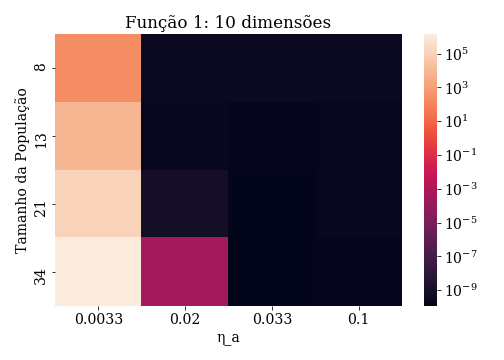
\includegraphics[width=2.0in]{figures/hiper_selection/function=01_dim=10.png}
\label{fig:func01dim10}}
\subfloat{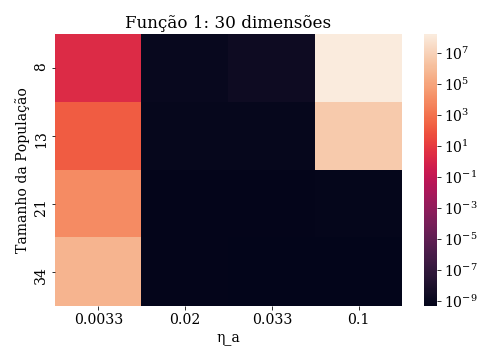
\includegraphics[width=2.0in]{figures/hiper_selection/function=01_dim=30.png}
\label{fig:func01dim30}}
\hfil
\subfloat{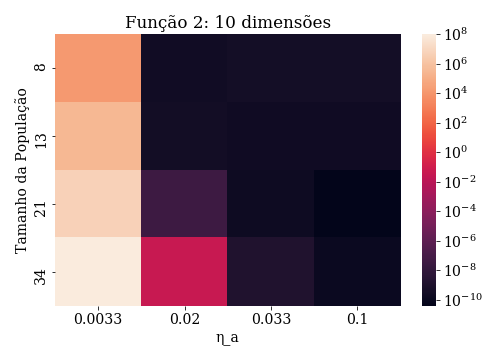
\includegraphics[width=2.0in]{figures/hiper_selection/function=02_dim=10.png}
\label{fig:func02dim10}}
\subfloat{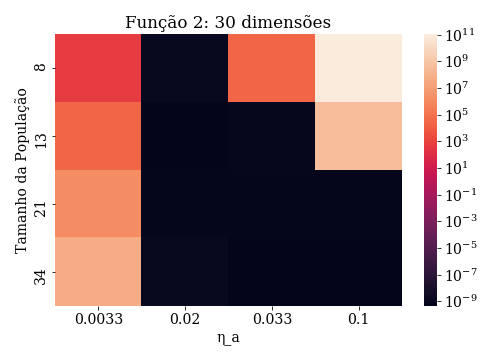
\includegraphics[width=2.0in]{figures/hiper_selection/function=02_dim=30.png}
\label{fig:func02dim30}}
\hfil
\subfloat{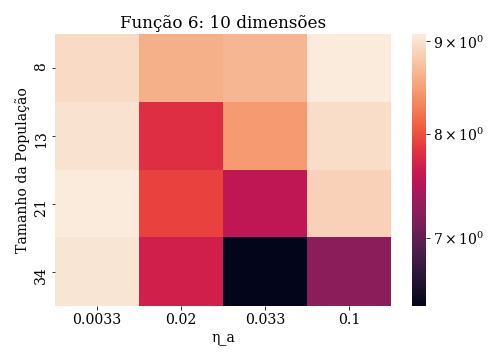
\includegraphics[width=2.0in]{figures/hiper_selection/function=06_dim=10.png}
\label{fig:func06dim10}}
\subfloat{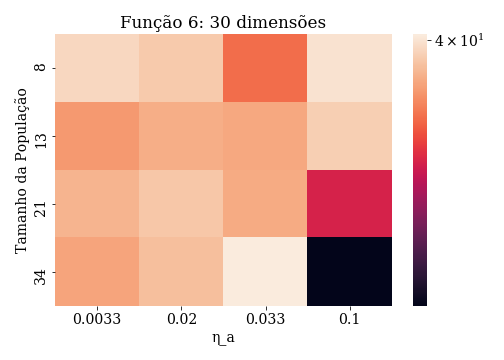
\includegraphics[width=2.0in]{figures/hiper_selection/function=06_dim=30.png}
\label{fig:func06dim30}}
\hfil
\subfloat{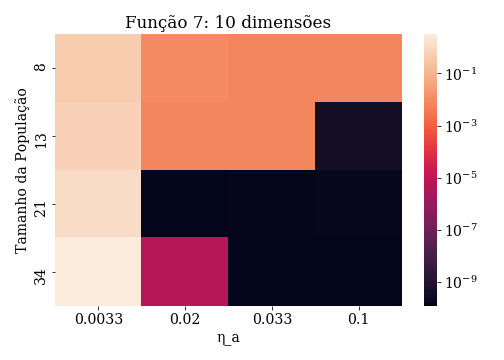
\includegraphics[width=2.0in]{figures/hiper_selection/function=07_dim=10.png}
\label{fig:func07dim10}}
\subfloat{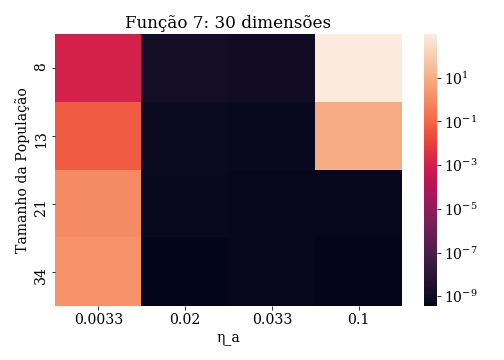
\includegraphics[width=2.0in]{figures/hiper_selection/function=07_dim=30.png}
\label{fig:func07dim30}}
\hfil
\subfloat{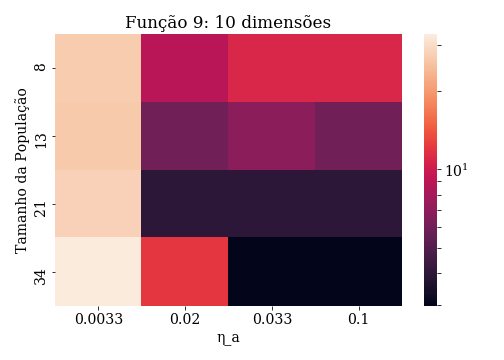
\includegraphics[width=2.0in]{figures/hiper_selection/function=09_dim=10.png}
\label{fig:func09dim10}}
\subfloat{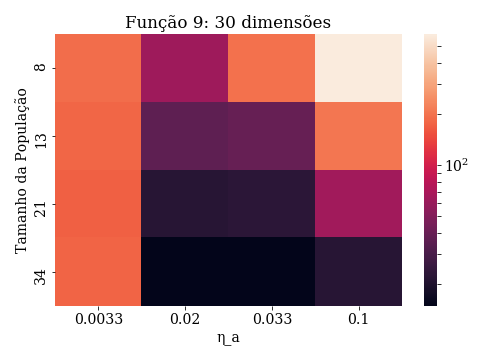
\includegraphics[width=2.0in]{figures/hiper_selection/function=09_dim=30.png}
\label{fig:func09dim30}}
\hfil
\subfloat{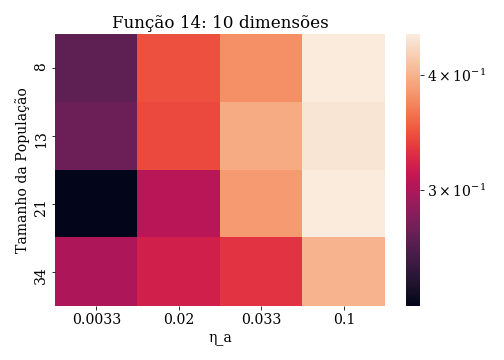
\includegraphics[width=2.0in]{figures/hiper_selection/function=14_dim=10.png}
\label{fig:func14dim10}}
\subfloat{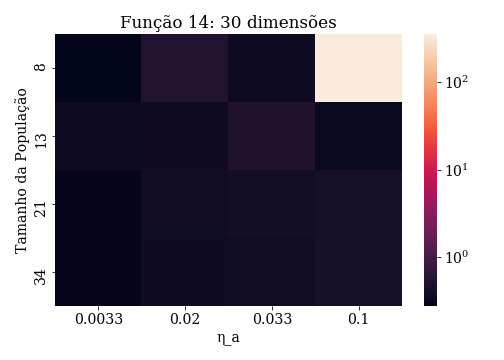
\includegraphics[width=2.0in]{figures/hiper_selection/function=14_dim=30.png}
\label{fig:func14dim30}}
\caption{Seleção de hiperparâmetros do xNES}
\label{fig:hiper}
\end{figure*}

Seguindo para a fase de comparação entre os algoritmos, a Figura~\ref{fig:comp} apresenta o erro de aptidão obtido por
cada algoritmo.
Nessa figura comparamos o xNES com os parâmetros selecionados na fase anterior, o xNES com valores originalmente
apresentados pelos autores e o CMA-ES também com seus valores padrão.
Assim como na etapa anterior, cada algoritmo foi rodado 51 vezes para cada função.
Os resultados também estão dispostos nas Tabelas~\ref{tab:results_xnes_10}, \ref{tab:results_xnes_30},
\ref{tab:results_xnes_orig_10}, \ref{tab:results_xnes_orig_10}, \ref{tab:results_cmaes_10} e \ref{tab:results_cmaes_30}.

A primeira consideração a se feita é que para as funções $1$ e $2$ todos algoritmos foram capazes de obter sucesso, ou seja,
erro menor que $10^{-8}$, dentro do número permitido de avaliações da função objetivo.
Observamos ainda nas funções $1$ e $2$ que o algoritmo xNES com parâmetros pré-selecionados apresentou menor média e
variância de aptidão.

Analisando a função $6$, ressalta-se que o algoritmo CMA-ES foi o único a conseguir obter sucesso no problema com $10$
dimensões, porém em apenas uma das 51 rodadas.
Considerando ainda as $10$ dimensões, o CMA-ES superou o xNES com valores originais, porém, esta dentro da margem de
erro do xNES com parâmetros selecionados, apesar de apresentar menor média de erro.
Por sua vez, para função $7$ com $30$ dimensões o CMA-ES superou os outros dois algoritmos que apresentaram resultados
iguais entre si.

A função $7$ apresenta um comportamento atípico, os resultados obtidos em $30$ dimensões para todos algoritmos foram superiores
aos resultados de $10$ dimensões.
Nesta função a variação de parâmetros do xNES se mostrou irrelevante.
Analisando o problema com 10 dimensões, o CMA-ES apresentou a maior média de erro e obteve sucesso apenas em 25\% das
rodadas enquanto os xNES obtiveram 50\% de sucesso, porém, os resultados ainda se encontram dentro da barra de erro.
Avaliando o problema com $30$ dimensões os xNES obtiveram sucesso em todos os casos enquanto o CMA-ES atingiu o 84\% das rodadas.

As funções $9$ e $14$ apresentam resultados parecidos entre todos algoritmos.
Nestas avaliações todos algoritmos apresentaram resultados dentro das margens de erro.

Os experimentos foram executados em um computador com 8 CPUs e totalizaram 50 minutos de processamento.

\begin{figure*}[!t]
\centering
\subfloat{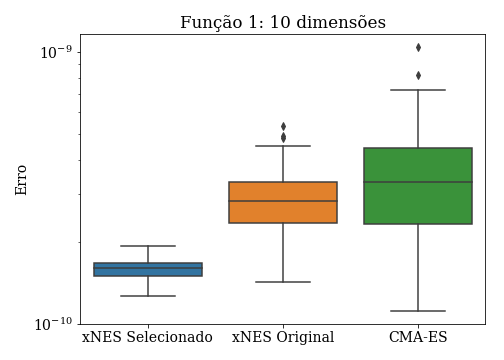
\includegraphics[width=2.0in]{figures/analysis_results/function=01_dim=10.png}
\label{fig:result_func01dim10}}
\subfloat{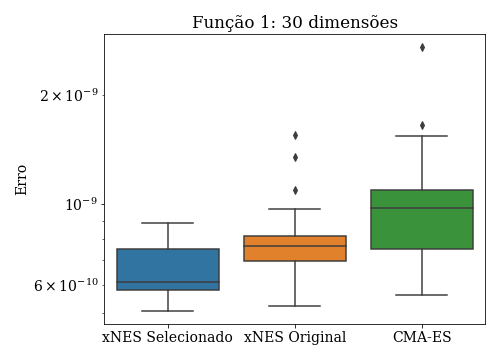
\includegraphics[width=2.0in]{figures/analysis_results/function=01_dim=30.png}
\label{fig:result_func01dim30}}
\hfil
\subfloat{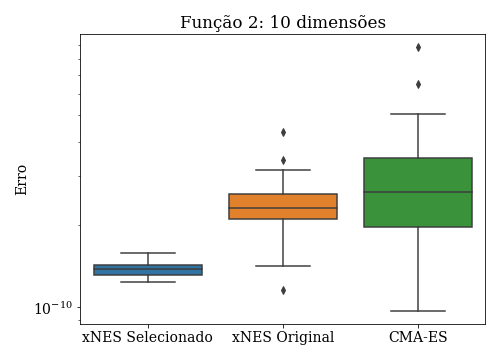
\includegraphics[width=2.0in]{figures/analysis_results/function=02_dim=10.png}
\label{fig:result_func02dim10}}
\subfloat{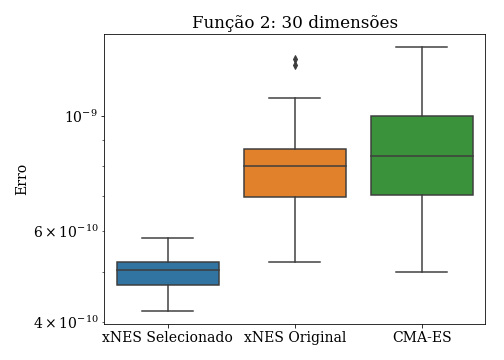
\includegraphics[width=2.0in]{figures/analysis_results/function=02_dim=30.png}
\label{fig:result_func02dim30}}
\hfil
\subfloat{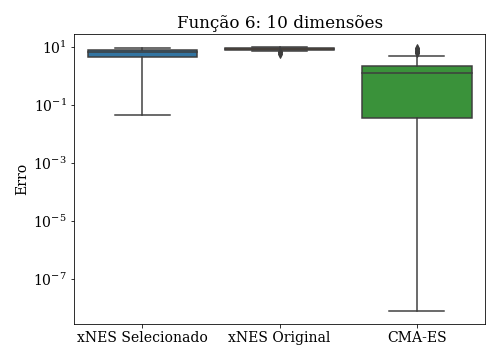
\includegraphics[width=2.0in]{figures/analysis_results/function=06_dim=10.png}
\label{fig:result_func06dim10}}
\subfloat{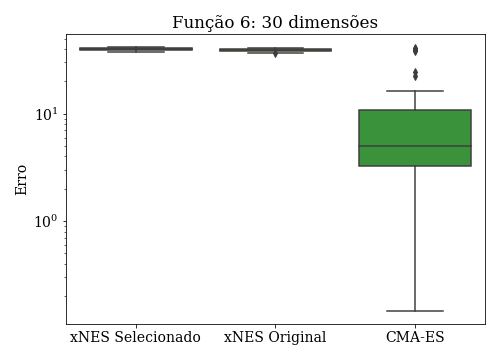
\includegraphics[width=2.0in]{figures/analysis_results/function=06_dim=30.png}
\label{fig:result_func06dim30}}
\hfil
\subfloat{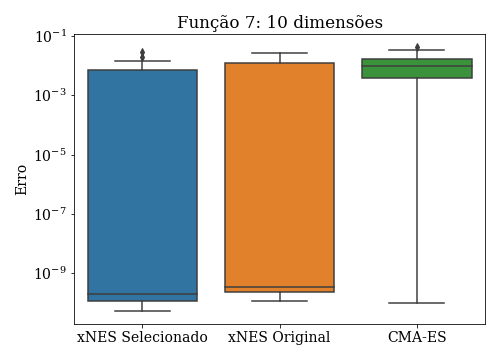
\includegraphics[width=2.0in]{figures/analysis_results/function=07_dim=10.png}
\label{fig:result_func07dim10}}
\subfloat{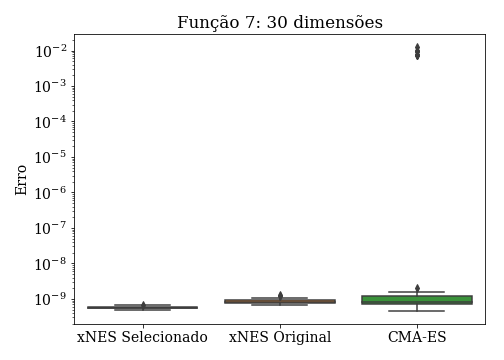
\includegraphics[width=2.0in]{figures/analysis_results/function=07_dim=30.png}
\label{fig:result_func07dim30}}
\hfil
\subfloat{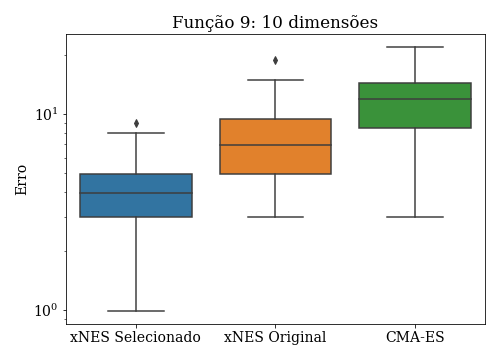
\includegraphics[width=2.0in]{figures/analysis_results/function=09_dim=10.png}
\label{fig:result_func09dim10}}
\subfloat{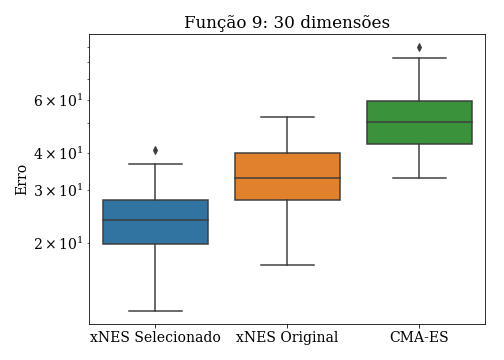
\includegraphics[width=2.0in]{figures/analysis_results/function=09_dim=30.png}
\label{fig:result_func09dim30}}
\hfil
\subfloat{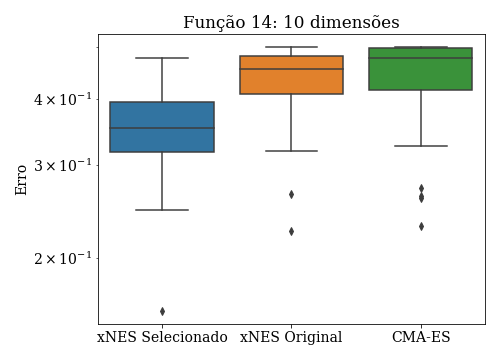
\includegraphics[width=2.0in]{figures/analysis_results/function=14_dim=10.png}
\label{fig:result_func14dim10}}
\subfloat{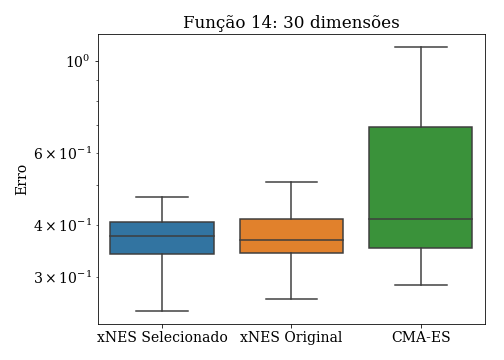
\includegraphics[width=2.0in]{figures/analysis_results/function=14_dim=30.png}
\label{fig:result_func14dim30}}
\caption{Comparação entre os algoritmos}
\label{fig:comp}
\end{figure*}


\begin{table}[!t]
\renewcommand{\arraystretch}{1.3}
\caption{xNES Selecionado - 10 Dimensões}
\label{tab:results_xnes_10}
\centering
\resizebox{\columnwidth}{!}{%
\begin{tabular}{|l|r|r|r|r|r|r|}
\hline
Função &    Melhor   &      Pior &   Mediana &     Média &  \specialcell{Desvio\\Padrão} &  \specialcell{Taxa de\\ Sucesso} \\
\hline
1        &  1.27e-10 &  1.93e-10 &  1.60e-10 &  1.60e-10 &      1.32e-11 &             1.00 \\
2        &  1.23e-10 &  1.58e-10 &  1.38e-10 &  1.38e-10 &      8.72e-12 &             1.00 \\
6        &  4.51e-02 &  9.39e+00 &  6.73e+00 &  6.09e+00 &      2.48e+00 &             0.00 \\
7        &  5.30e-11 &  2.96e-02 &  2.01e-10 &  4.98e-03 &      6.21e-03 &             0.51 \\
9        &  9.95e-01 &  8.95e+00 &  3.98e+00 &  4.14e+00 &      1.81e+00 &             0.00 \\
14       &  1.59e-01 &  4.77e-01 &  3.52e-01 &  3.49e-01 &      6.10e-02 &             0.00 \\
\hline
\end{tabular}
}
\end{table}

\begin{table}[!t]
\renewcommand{\arraystretch}{1.3}
\caption{xNES Selecionado - 30 Dimensões}
\label{tab:results_xnes_30}
\centering
\resizebox{\columnwidth}{!}{%
\begin{tabular}{|l|r|r|r|r|r|r|}
\hline
Função &    Melhor   &      Pior &   Mediana &     Média &  \specialcell{Desvio\\Padrão} &  \specialcell{Taxa de\\ Sucesso} \\
\hline
1        &  5.09e-10 &  8.84e-10 &  6.12e-10 &  6.60e-10 &       1.04e-10 &              1.00 \\
2        &  4.21e-10 &  5.82e-10 &  5.04e-10 &  4.98e-10 &       3.68e-11 &              1.00 \\
6        &  3.75e+01 &  4.16e+01 &  3.97e+01 &  3.97e+01 &       1.05e+00 &              0.00 \\
7        &  4.86e-10 &  6.92e-10 &  5.65e-10 &  5.75e-10 &       4.89e-11 &              1.00 \\
9        &  1.19e+01 &  4.08e+01 &  2.39e+01 &  2.44e+01 &       6.47e+00 &              0.00 \\
14       &  2.48e-01 &  4.69e-01 &  3.77e-01 &  3.72e-01 &       4.94e-02 &              0.00 \\
\hline
\end{tabular}
}
\end{table}

\begin{table}[!t]
\renewcommand{\arraystretch}{1.3}
\caption{xNES Original - 10 Dimensões}
\label{tab:results_xnes_orig_10}
\centering
\resizebox{\columnwidth}{!}{%
\begin{tabular}{|l|r|r|r|r|r|r|}
\hline
Função &    Melhor   &      Pior &   Mediana &     Média &  \specialcell{Desvio\\Padrão} &  \specialcell{Taxa de\\ Sucesso} \\
\hline
1        &  1.42e-10 &  5.34e-10 &  2.82e-10 &  2.98e-10 &      8.84e-11 &             1.00 \\
2        &  1.16e-10 &  4.34e-10 &  2.30e-10 &  2.37e-10 &      5.39e-11 &             1.00 \\
6        &  5.95e+00 &  9.91e+00 &  8.79e+00 &  8.59e+00 &      8.29e-01 &             0.00 \\
7        &  1.14e-10 &  2.71e-02 &  3.46e-10 &  6.13e-03 &      7.42e-03 &             0.51 \\
9        &  2.98e+00 &  1.89e+01 &  6.96e+00 &  7.53e+00 &      3.45e+00 &             0.00 \\
14       &  2.24e-01 &  5.00e-01 &  4.55e-01 &  4.38e-01 &      6.00e-02 &             0.00 \\
\hline
\end{tabular}
}
\end{table}

\begin{table}[!t]
\renewcommand{\arraystretch}{1.3}
\caption{xNES Original - 30 Dimensões}
\label{tab:results_xnes_orig_30}
\centering
\resizebox{\columnwidth}{!}{%
\begin{tabular}{|l|r|r|r|r|r|r|}
\hline
Função &    Melhor   &      Pior &   Mediana &     Média &  \specialcell{Desvio\\Padrão} &  \specialcell{Taxa de\\ Sucesso} \\
\hline
1        &  5.23e-10 &  1.54e-09 &  7.66e-10 &  7.83e-10 &       1.73e-10 &              1.00 \\
2        &  5.22e-10 &  1.29e-09 &  7.99e-10 &  7.98e-10 &       1.50e-10 &              1.00 \\
6        &  3.65e+01 &  4.12e+01 &  3.96e+01 &  3.94e+01 &       1.08e+00 &              0.00 \\
7        &  6.62e-10 &  1.28e-09 &  8.43e-10 &  8.52e-10 &       1.27e-10 &              1.00 \\
9        &  1.69e+01 &  5.27e+01 &  3.28e+01 &  3.43e+01 &       8.65e+00 &              0.00 \\
14       &  2.64e-01 &  5.09e-01 &  3.68e-01 &  3.87e-01 &       7.12e-02 &              0.00 \\
\hline
\end{tabular}
}
\end{table}

\begin{table}[!t]
\renewcommand{\arraystretch}{1.3}
\caption{CMA-ES - 10 Dimensões}
\label{tab:results_cmaes_10}
\centering
\resizebox{\columnwidth}{!}{%
\begin{tabular}{|l|r|r|r|r|r|r|}
\hline
Função &    Melhor   &      Pior &   Mediana &     Média &  \specialcell{Desvio\\Padrão} &  \specialcell{Taxa de\\ Sucesso} \\
\hline
1        &  1.12e-10 &  1.04e-09 &  3.31e-10 &  3.57e-10 &       1.80e-10 &             1.00 \\
2        &  9.73e-11 &  8.84e-10 &  2.64e-10 &  2.88e-10 &       1.39e-10 &             1.00 \\
6        &  7.88e-09 &  9.13e+00 &  1.24e+00 &  2.06e+00 &       2.49e+00 &             0.02 \\
7        &  9.66e-11 &  4.18e-02 &  9.86e-03 &  1.16e-02 &       1.03e-02 &             0.25 \\
9        &  2.98e+00 &  2.19e+01 &  1.19e+01 &  1.16e+01 &       4.64e+00 &             0.00 \\
14       &  2.30e-01 &  5.00e-01 &  4.77e-01 &  4.44e-01 &       7.38e-02 &             0.00 \\
\hline
\end{tabular}
}
\end{table}

\begin{table}[!t]
\renewcommand{\arraystretch}{1.3}
\caption{CMA-ES - 30 Dimensões}
\label{tab:results_cmaes_30}
\centering
\resizebox{\columnwidth}{!}{%
\begin{tabular}{|l|r|r|r|r|r|r|}
\hline
Função &    Melhor   &      Pior &   Mediana &     Média &  \specialcell{Desvio\\Padrão} &  \specialcell{Taxa de\\ Sucesso} \\
\hline
1        &  5.60e-10 &  2.70e-09 &  9.74e-10 &  9.84e-10 &       3.43e-10 &             1.00 \\
2        &  5.00e-10 &  1.36e-09 &  8.35e-10 &  8.63e-10 &       2.06e-10 &             1.00 \\
6        &  1.47e-01 &  4.10e+01 &  5.04e+00 &  9.99e+00 &       1.20e+01 &             0.00 \\
7        &  4.65e-10 &  1.23e-02 &  8.22e-10 &  1.40e-03 &       3.35e-03 &             0.84 \\
9        &  3.28e+01 &  8.95e+01 &  5.07e+01 &  5.27e+01 &       1.31e+01 &             0.00 \\
14       &  2.87e-01 &  1.08e+00 &  4.15e-01 &  5.14e-01 &       2.00e-01 &             0.00 \\
\hline
\end{tabular}
}
\end{table}


\section{Conclusões} \label{sec:conclusion}
Concluímos que a seleção de parâmetros do xNES foi capaz de apresentar resultados equivalentes ou superiores aos
parâmetros padrão, sendo o tamanho da população consideravelmente maior do que o proposto originalmente.
Comparando o xNES com parâmetros selecionados com o CMA-ES observamos que em praticamente todos os casos os algoritmos
obtiveram resultados equivalentes, ficando dentro da margem de erro.

Os algoritmos apresentaram performance muito semelhantes entre si, este fato pode ser explicado devido a semelhança entre
os dois algoritmos, sendo o método de estimação da matriz de covariância sua única diferença relevante.

Os algoritmos se mostraram eficientes computacionalmente, necessitando de pouco tempo de processamento e memória.
Desta forma, avalia-se que são boas escolhas para otimização de funções reais.



% trigger a \newpage just before the given reference
% number - used to balance the columns on the last page
% adjust value as needed - may need to be readjusted if
% the document is modified later
%\IEEEtriggeratref{8}
% The "triggered" command can be changed if desired:
%\IEEEtriggercmd{\enlargethispage{-5in}}

% references section

% can use a bibliography generated by BibTeX as a .bbl file
% BibTeX documentation can be easily obtained at:
% http://mirror.ctan.org/biblio/bibtex/contrib/doc/
% The IEEEtran BibTeX style support page is at:
% http://www.michaelshell.org/tex/ieeetran/bibtex/
%\bibliographystyle{IEEEtran}
% argument is your BibTeX string definitions and bibliography database(s)
%\bibliography{IEEEabrv,../bib/paper}
%
% <OR> manually copy in the resultant .bbl file
% set second argument of \begin to the number of references
% (used to reserve space for the reference number labels box)

\bibliographystyle{IEEEtran}
\bibliography{bibliography}

\end{document}
